\documentclass[nouppercase]{ifmbe}


\title{Preliminary Results of 3D Slicer localization to Portuguese and Spanish for the Latin American Biomedical Engineering Community}

\affiliation{Brigham and Women’s Hospital, Harvard Medical School, Boston, MA, USA }{HMS}
\affiliation{Department of Computing and Mathematics, University of São Paulo, Ribeirão Preto, Brazil}{USP}
\affiliation{Universidad Autónoma del Estado de México, Toluca, México}{UAEMEX}
\affiliation{Queen’s University, Kingston, ON, Canada}{QU}
\affiliation{Isomics Inc., Cambridge, MA, USA}{ISO}


\author{Sonia Pujol}{HMS}
\author{Paulo Eduardo de Barros}{USP}
\author{Valeria Gómez-Valdes}{UAEMEX}
\author{Lucas Sanchez Silva}{USP}
\author{Douglas Gonçalves}{USP}
\author{João Pedro Alves Januário}{USP}
\author{Victor M. Montãno Serrano}{UAEMEX}
\author{Enrique Hernandez-Laredo}{UAEMEX}
\author{Monserrat Ríos-Hernández}{UAEMEX}
\author{Andras Lasso}{QU}
\author{Steve Pieper}{ISO}
\author{Ron Kikinis}{HMS}
\author{Adriana Vilchis González}{UAEMEX}
\author{Luiz Otavio Murta Junior}{USP}


\begin{document}

\maketitle

\begin{abstract}
3D Slicer is an open source software platform for medical image analysis and image-guided intervention used in medical research around the world. However, until recently, the platform was available in the English language only. This paper presents our work on localizing 3D Slicer to Portuguese and Spanish to facilitate access to the platform to the Latin American biomedical research community. We used the 3D Slicer Weblate repository and the 3D Slicer Language Packs Extension to translate the user interface and glossary of the platform. 
\end{abstract}

\begin{keywords}
3D Slicer; Software Localization; Medical Image Computing
\end{keywords}

\section{Introduction}

Open source software provides essential resources to the biomedical research community for advancing health. With over 20 years of development, 3D Slicer stands as a robust platform for medical image analysis and image-guided intervention \cite{SLICER}. We introduced the platform and examples of clinical research applications developed using the software to the Latin American biomedical research community during a workshop at the joint IX Latin American Congress on Biomedical Engineering (CLAIB 2022) and the XXVIII Brazilian Congress on Biomedical Engineering (CBEB 2022) \cite{CLAIB-CBEB-2022}. 

However, 3D Slicer was initially developed in English, potentially limiting accessibility for researchers in non-English speaking countries. In order to facilitate access to the platform for biomedical researchers in Latin America, we have engaged in a localization effort to translate the user interface and documentation to Portuguese and Spanish. The paper presents our preliminary work on the localization of the 3D Slicer for Latin America. 

\section{Materials and Methods}

We used the web-based 3D Slicer Weblate translation repository and the 3D Slicer Language Packs extension to localize the user interface elements of 3D Slicer to Brazilian Portuguese and Latin American Spanish \cite{LANGUAGEPACK, WEBLATE}. Additionally, to provide a reference to end-users unfamiliar with 3D Slicer terminology, we translated the 3D Slicer glossary of medical image computing terms \cite{GLOSSARY}. Furthermore, we translated the documentation of the 3D Slicer Language Packs extension into both languages to facilitate access to the localized version of the software for the Latin American biomedical research community, enabling their contribution to future translation.

\section{Results and Discussion}

The translation of the 3D Slicer user interface to Portuguese and Spanish encompasses over 5,300 strings in each language. Figures \ref{fig:portuguese} and \ref{fig:spanish} showcase the Volumes module of 3D Slicer translated into Portuguese and Spanish, respectively. We translated the documentation for the Slicer Language Packs extension and the 3D Slicer glossary and made them available on GitHub \cite{PORTUGUESE-GLOSSARY, SPANISH-GLOSSARY}. The initial project outcomes were presented at the 39th edition of the Slicer Project Week hackathon, a bi-annual event that brings where we received valuable feedback from the 3D Slicer community \cite{SLICER-FOR-LA-PW39}.

\begin{figure}[ht]
      \centering
          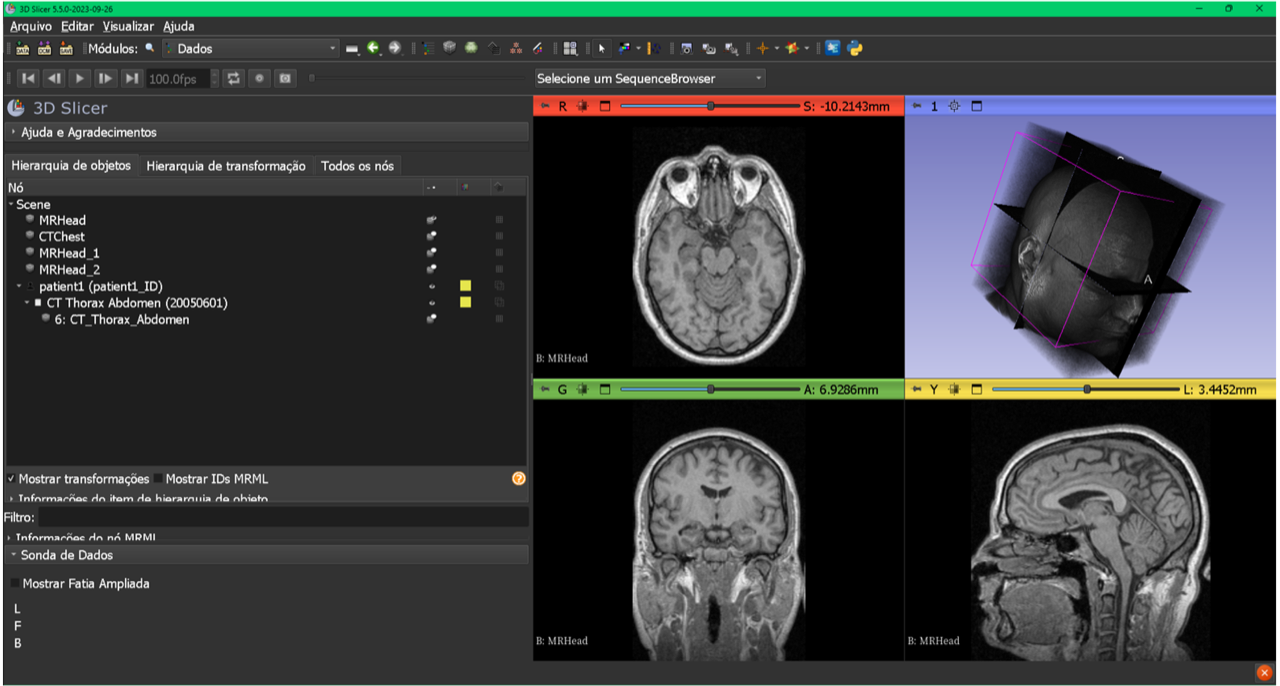
\includegraphics[width=1\columnwidth]{figures/3DSlicer_Portuguese.png}
      \caption{Volumes module of 3D Slicer translated to Portuguese, where one can see both the core 3D Slicer and the module graphical user interface in Portuguese.}
      \label{fig:portuguese}
\end{figure}

\begin{figure}[ht]
      \centering
          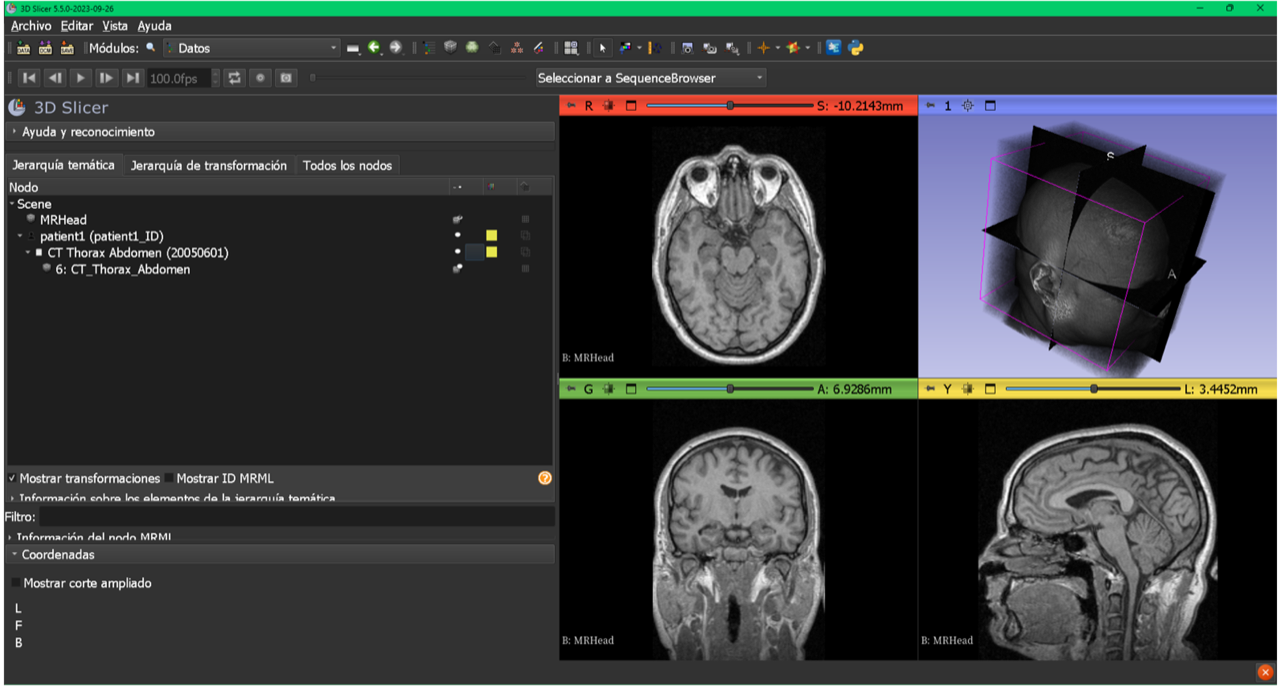
\includegraphics[width=1\columnwidth]{figures/3DSlicer_Spanish.png}
      \caption{Volumes module of 3D Slicer translated to Spanish, where one can see both the core 3D Slicer and the module graphical user interface in Spanish.}
      \label{fig:spanish}
\end{figure}

\section{Conclusions}

We have created the first localized version of 3D Slicer in Portuguese and Spanish for Latin America. This initiative enables researchers across the region to fully utilize the platform. Future plans include maintaining these translations and expanding them to encompass additional modules and resources, fostering a more inclusive and collaborative research environment for the Latin American biomedical engineering community.

\section*{Acknowledgements}

This project has been made possible in part by grants number 2021-237549 and 2022-252572 from the Chan Zuckerberg Initiative DAF, an advised fund of the Silicon Valley Community Foundation.

\bibliography{CBEB}

\end{document}
